\section{Dados Semi-Estruturados}

Podemos dividir um banco de dados tradicional em duas partes: seu esquema e seus dados. O esquema é todo o esqueleto do banco, que descreve as tabelas, as chaves e todo o resto da estruturação, enquanto os dados são as entradas armazenadas. Todavia, existem dados cuja natureza \textit{não é} estruturada. Dados não estruturados são aqueles no qual a estrutura está contida dentro dos próprios dados \cite{buneman1997semistructured}. O principal exemplo de dados semi-estruturados é a própria internet, pois os dados não seguem necessariamente um padrão, e podem ter diversos níveis de organização diferentes. Outros exemplos menos diretos são binários executáveis, pacotes TCP/IP e arquivos compactados \cite{geeks}.
Uma definição simples e direta de dado semi-estruturado é: dados que de um ponto de vista prático não são nem crus nem estritamente tipado através de tabelas ou grafos \cite{abiteboul1997querying}.

Existem diversas características que diferem os dados semi-estruturados dos dados organizados da maneira clássica \cite{dosdados}. Esse tipo de dado normalmente possui a estrutura definida após eles já existirem, ou seja, apesar de nem sempre existir algum esquema implícito, é possível extrair alguma organização dos dados apresentados. Apesar disso, a estrutura é irregular, pois dados similares não necessariamente respeitam a mesma organização. Essa organização, que pode ser implícita ou explícita, as vezes compreende apenas alguma parte do dado, uma vez que não existem restrições para a estruturação (nada obriga que todo o documento respeite as classificações definidas). Além disso, a estrutura é extensa, uma vez que os dados são heterogêneos, e evolucionária, pois seus valores mudam constantemente (especialmente no caso da web). Por fim, uma de suas características mais marcantes é que os dados se misturam com a estrutura, e não é possível ter uma distinção clara desses dois elementos. 

\begin{figure}[t]
    \centering
    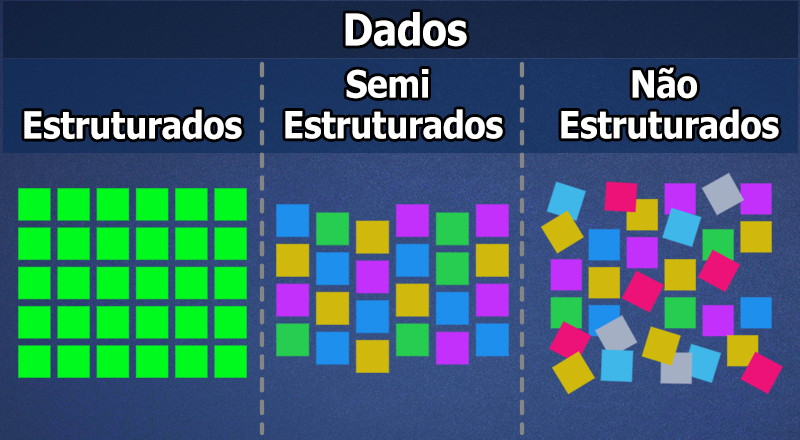
\includegraphics[width=\textwidth]{imagens/tipos.jpg}
    \caption{Distinção entre dados estruturados, semi-estruturados e não estruturados. Fonte: https://universidadedatecnologia.com.br/dados-estruturados-e-nao-estruturados/}
    \label{fig:dados}
\end{figure}

A tabela 1, retirada do artigo de Mello et. al. \cite{dosdados} expõem as diferenças entre os bancos de dados semi-estruturados e os bancos de dados estruturados.


% Tabela gerada no site: https://www.tablesgenerator.com/
\begin{table}[]
\centering
\resizebox{\textwidth}{!}{\begin{tabular}{|c|c|}
\hline
\rowcolor[HTML]{CBCEFB} 
\textbf{Dados tradicionais}              & \textbf{Dados semi-estruturados}             \\ \hline
Esquema predefinido                      & Nem sempre há um esquema predefinido         \\ \hline
Estrutura regular                        & Estrutura irregular                          \\ \hline
Estrutura independente dos dados         & Estrutura embutida no dado                   \\ \hline
Estrutura reduzida                       & Estrutura extensa                            \\ \hline
Estrutura fracamente evolutiva           & Estrutura fortemente evolutiva               \\ \hline
Estrutura prescritiva                    & Estrutura descritiva                         \\ \hline
Distinção entre estrutura e dado é clara & Distinção entre estrutura e dado não é clara \\ \hline
\end{tabular}}
\caption{Diferenças entre dados tradicionais e dados semi-estruturados \cite{dosdados}.}
\label{tab:my-table}
\end{table}

O uso de dados semi-estruturados permite que os desenvolvedores integrem diversos sistemas e integrem diversos fluxos de dados, uma vez que a estrutura desse tipo de dado é flexível. Como sites e APIs podem evoluir rapidamente com o tempo, o uso de dados semi-estruturados garante que a integração seja contínua, pois sua estrutura é evolutiva \cite{treehouse}.

Apesar de ser uma ferramenta poderosa, os dados semi-estruturados possuem vantagens e desvantagens em relação aos dados estruturados. As principais vantagens já foram citadas, como a capacidade de suportar diversas fontes de dados e a evolução de seus formatos. Já entre as desvantagens, podemos citar a dificuldade que existe para realizar consultas de maneira eficiente, tanto que consultas em bancos semi-estruturados são uma linha de pesquisa por si só (ao contrário de dados tradicionais, que possuem o SQL como linguagem padrão bem implementada e otimizada). Além disso, como as restrições do esquema não existem para os dados semi-estruturados, o banco está mais propenso a receber dados corrompidos, incorretos e todo o tipo de lixo. Portanto, é necessário ter cuidado ao escolher utilizar esse tipo de banco de dados, e manter a atenção para esses detalhes durante a implementação do aplicativo que utilizará a base.

Para exemplificar os bancos de dados semi-estruturados e demonstrar seu uso prático, apresentaremos duas linguagens capazes de descrever dados dessa maneira, o XML e o JSON.
